\documentclass[a5paper,12pt,french]{book}
\usepackage[margin=2cm,landscape]{geometry}
\usepackage[thinfonts]{uglix2}
\usepackage{circuitikz}
\pagestyle{empty}
\begin{document}
\chapter*{Logique}

\section{Du transistor à l'ordinateur}

Le transistor est à la base de la plupart des composants d'un ordinateur. Pour faire simple c'est un composant avec une entrée, une sortie, et une alimentation.Quand il est alimenté, le transistor laisse passer le courant de l'entrée vers la sortie et dans le cas contraire le courant ne passe pas.\\
C'est l'élément de base des \textit{circuits logiques}. 

\newpage
\begin{definition}[ : circuit logique]
	Un circuit logique prend en entrée un ou plusieurs signaux électriques. Chacun de ses signaux peut être dans l'état 0 ou l'état 1.\\
	En sortie, le circuit logique produit un signal (0 ou 1) obtenu en appliquant des \textit{opérations booléennes} aux signaux d'entrée.
\end{definition}

Un circuit logique est une implémentation matérielle d'une \textit{fonction logique}. La fonction logique est, quant à elle, la version \og mathématique\fg{} du circuit. Nous confondrons ces deux notions par la suite.
\newpage
\subsection{Opérateurs logiques de base}

À l'aide des opérateurs suivants, on peut construire toutes les fonctions logiques.
\newpage
\subsubsection*{L'opérateur \og non\fg{}}

C'est un opérateur \textbf{unaire} : il ne prend qu'une seule variable booléenne en entrée.\\

\double{
	\textbf{Table de valeurs}\\}
{
	\textbf{Symbole de porte logique européen}\\}{11.5cm}
\double{
	\begin{tabular}{|c|c|}
		\hline\rowcolor{lightgray}
		x & \textit{non} x \\
		\hline
		0 & 1               \\
		\hline
		1 & 0               \\
		\hline
\end{tabular}}
{
	\tikz{\draw (0,0) node[european not port]{};}}{11.5cm}

Cet opérateur renvoie \og le contraire de ce qu'il a reçu\fg{}.\\
Parmi les notations que l'on rencontre pour noter \og non x\fg{} il y a
\begin{enumerate}[\textbullet]
	\item 	 \tw{NOT x}
	\item 	$\barmin{x}$
	\item 	$!x$
\end{enumerate}
\newpage

\subsubsection*{L'opérateur \og et\fg{}}

C'est un opérateur \textbf{binaire} : il prend deux variables booléennes en entrée.\\

\double{
	\textbf{Table de valeurs}\\}
{
	\textbf{Symbole de porte logique européen}\\}{11.5cm}
\double{
	\begin{tabular}{|c|c|c|}
		\hline\rowcolor{lightgray}
		x & y & x \textit{et} y \\
		\hline
		0 & 0 & 0               \\
		\hline
		0 & 1 & 0               \\
		\hline
		1 & 0 & 0               \\
		\hline
		1 & 1 & 1               \\
		\hline
\end{tabular}}
{
	\tikz{\draw (0,0) node[european and port]{};}}{11.5cm}

Un \og et\fg{} ne renvoie vrai que si ses deux entrées sont vraies.\\
Parmi les notations que l'on rencontre pour noter \og x et y\fg{} il y a 
\begin{enumerate}[\textbullet]
	\item 	 \tw{x AND y}
	\item 	$x\wedge y$	
	\item 	$x \&\& y$
\end{enumerate}

\subsubsection*{L'opérateur \og ou\fg{}}

C'est également un opérateur \textbf{binaire}.\\

\double{
	\textbf{Table de valeurs}\\}
{
	\textbf{Symbole de porte logique européen}\\}{11.5cm}
\double{
	\begin{tabular}{|c|c|c|}
		\hline\rowcolor{lightgray}
		x & y & x \textit{ou} y \\
		\hline
		0 & 0 & 0               \\
		\hline
		0 & 1 & 1               \\
		\hline
		1 & 0 & 1               \\
		\hline
		1 & 1 & 1               \\
		\hline
\end{tabular}}
{
	\tikz{\draw (0,0) node[european or port]{};}}{11.5cm}

Un \og ou\fg{} ne renvoie faux que si ses deux entrées sont fausses.\\
Parmi les notations que l'on rencontre pour noter \og x ou y\fg{} il y a

\begin{enumerate}[\textbullet]
	\item 	 \tw{x OR y}
	\item 	$x\vee y$	
	\item 	$x || y$
\end{enumerate}

On peut montrer qu'il est possible de se passer de la fonction \textit{et} et que toutes les fonctions logiques peuvent s'écrire à l'aide de 
fonctions \textit{non} et \textit{ou} (on peut même n'utiliser qu'une seule fonction : la fonction \og non ou\fg{}). Le choix de ces trois fonctions 
\textit{et}, \textit{ou} et \textit{non} est donc, en quelque sorte, arbitraire.

\begin{definition}[ : \'Equivalence de deux circuits/fonctions logiques]
	On dira que deux fonctions logiques sont équivalentes lorsqu'elles prennent le même nombre de variables en entrée (le même nombre de signaux si on parle de circuits) et si ces deux fonctions donnent le même résultat lorsque les variables d'entrées ont les mêmes valeurs : on dit que les fonctions ont même \textit{table de vérité}.
	Lorsque deux fonctions logiques sont équivalentes, on dit aussi que leurs expressions booléennes sont équivalentes.
\end{definition}

\newpage
\begin{exemple}[s]
	\begin{enumerate}[\textbullet]
		\item 		Les expressions booléennes $$not(A\ and\ B)$$ et $$(not\ A)\ or\ (not\ B)$$ sont équivalentes.\\
		Pour le prouver il suffit de vérifier que leurs tables de vérité sont les mêmes : on fait varier les valeurs de A et de B selon toutes les possibilités et on regarde le résultat de chaque expression.
		\begin{center}
			\begin{tabular}{|c|c|c|c|}
				\hline\rowcolor{lightgray}
				A 	& B 	&  A and B	& not (A and B) \\
				\hline
				0 	& 0 	& 	0   	& \cellcolor{orange@color!25}	1         \\
				\hline
				0 	& 1 	& 	0   	& \cellcolor{orange@color!25}	1         \\
				\hline
				1 	& 0 	& 	0   	& \cellcolor{orange@color!25}	1         \\
				\hline
				1 	& 1 	& 	1   	& \cellcolor{orange@color!25}	0         \\
				\hline
			\end{tabular}\hspace{2em}
			\begin{tabular}{|c|c|c|c|c|}
				\hline\rowcolor{lightgray}
				A 	& B 	&  not A & not B	& (not A) or (not B)  \\
				\hline
				0 	& 0 	& 	1   & 	1       & \cellcolor{orange@color!25}	1\\
				\hline
				0 	& 1 	& 	1   & 	0       & \cellcolor{orange@color!25}	1\\
				\hline
				1 	& 0 	& 	0   & 	1       & \cellcolor{orange@color!25}	1\\
				\hline
				1 	& 1 	& 	0   & 	0 		&\cellcolor{orange@color!25}  0 \\
				\hline
			\end{tabular}
		\end{center}
		Les dernières colonnes de chaque tableau sont les mêmes : les expressions sont donc équivalentes.
		\item 	En procédant de même on montre très facilement que \og non non x\fg{} et \og x\fg{} sont équivalentes.	
	\end{enumerate}

\end{exemple}

\begin{exercice}[]
	Montrer que  $$not(A\ or\ B)$$ et $$(not\ A)\ and\ (not\ B)$$ sont équivalentes.\\
\end{exercice}

\begin{exercice}[]
	On peut définir le \og ou exclusif\fg{} noté xor comme ceci :  A xor B n'est vrai que si A est vrai ou B est vrai, mais pas les deux.
	\begin{enumerate}[\bfseries 1.]
		\item 	Donner la table de vérité de xor.
		\item 	Montrer que A xor B équivaut à (A or B) and (not(A and B)).
		\item 	Montrer que A xor B équivaut à (A and (not B) ) or ( (not A) and B).
		\item 	Représenter A xor B avec un circuit logique, en utilisant les symboles de porte logique européens.
	\end{enumerate}
\end{exercice}
\newpage
\begin{exercice}[]
	On définit l'opération \og nor\fg{}, notée $\downarrow$ par : $$A\downarrow B = not(A\ or\ B)$$
	
	Cette opération est dite \textit{universelle} car elle permet de retrouver toutes les autres opérations.
	
	\begin{enumerate}[\bfseries 1.]
		\item 	\'Ecrire la table de vérité de nor.
		\item 	Montrer que $A\downarrow A = not\ A$.
		\item 	En utilisant les exemples de la page précédente, en déduire que $(A\downarrow B)\downarrow(A\downarrow B) = A\ or\ B$.
		\item 	Comment à partir de A, B et $\downarrow$ obtenir $A\ and\ B$ ?
	\end{enumerate}
\end{exercice}
\newpage
\subsection{Un exemple détaillé : le multiplexeur}

Il s'agit d'une fonction très importante : soient A, B et C trois variables logiques, alors m(A,B,C)=B si A vaut 0 et C si A vaut 1.\\ m permet 
donc de sélectionner B ou C suivant la valeur de A. Voici la table de valeurs de m :
\begin{center}
	\begin{tabular}{|c|c|c|c|}
		\hline
		A & B & C & m(A,B,C) \\
		\hline
		0 & 0 & 0 & 0        \\
		\hline
		0 & 0 & 1 & 0        \\
		\hline
		0 & 1 & 0 & 1        \\
		\hline
		0 & 1 & 1 & 1        \\
		\hline
		1 & 0 & 0 & 0        \\
		\hline
		1 & 0 & 1 & 1        \\
		\hline
		1 & 1 & 0 & 0        \\
		\hline
		1 & 1 & 1 & 1        \\
		\hline
	\end{tabular}
\end{center}

On va décomposer m à l'aide des opérateurs de base. Ici, un raisonnement simple permet d'y arriver :
\begin{itemize}
	\item quand A vaut 0, on peut garder la valeur de B en faisant (\textit{non} A) \textit{et} B;
	\item quand A vaut 1, on peut garder la valeur de C en faisant A \textit{et} C;
	\item il se trouve que ces deux observations vont bien ensemble car quand A vaut 0, A \textit{et} C vaut automatiquement 0, et quand A vaut 
	1, (\textit{non} A) \textit{et} B vaut automatiquement 0;
	\item on en conclut que l'\textbf{expression symbolique} de m est m(A,B,C) =  (A \textit{et} C) ou ((\textit{non} A)  \textit{et} B).
\end{itemize}
Le circuit logique modélisant m est le suivant :
\begin{center}
	\begin{tikzpicture}[yscale=.7]
	\coordinate (A) at (0,4);
	\draw (A) node[left]{A}	\ball ;
	\coordinate (B) at (0,2);
	\draw (B) node[left]{B}	\ball ;
	\coordinate (C) at (0,0);
	\draw (C) node[left]{C}	\ball ;
	\node[european not port] (not1) at (2,4) {};
	\node[european and port] (and1) at (5,3) {};
	\node[european and port] (and2) at (5,1) {};
	\node[european or port] (or1) at (8,2) {};
	\draw (and1.out) |- (or1.in 1) (and2.out) |- (or1.in 2);
	\draw (C) |- (and2.in 2);
	\draw (B) |- (and1.in 2);
	\draw (not1.out) |- (and1.in 1);
	\draw (A) |- (not1.in);
	\draw (0.5,4)|- (and2.in 1);
	\draw (or1.out) \ball node[right]{m(A,B,C)};
	\end{tikzpicture}
\end{center}

\begin{exercice}[]
	On veut construire un \og additionneur\fg{} selon le principe suivant :
	\begin{enumerate}[\textbullet]
		\item 	A et B représentent deux bits à ajouter
		\item 	S et R sont respectivement
			\begin{enumerate}[-]
				\item 	la somme (sur un bit, donc) de A et B;
				\item 	la retenue.	
			\end{enumerate} 
	\end{enumerate}
	Par exemple si A et B valent 1, alors S vaudra 0 et R vaudra 1.
	\begin{enumerate}[\bfseries 1.]
		\item 	Donner les tables de vérités de R et de S.
		\item 	Exprimer R et S en fonction de A et B et des opérations \og non\fg{}, \og ou\fg{} et \og et\fg{}.
		\item 	Représenter R et S avec un (ou des) circuit(s) logique(s), en utilisant les symboles de porte logique européens.
	\end{enumerate}
\end{exercice}
\begin{exercice}
     Pour chiffrer un message, une méthode, dite du masque jetable, consiste à le combiner avec une chaîne de caractères de longueur comparable.
     Une implémentation possible utilise l’opérateur \texttt{XOR} (ou exclusif) dont voici la table de vérité :
    \begin{center}
    	\begin{tabular}{|c|c|c|}
                \hline
                \rowcolor{UGLiOrange} \textbf{\color{white}\texttt{a} }& \textbf{\color{white}\texttt{b}} & \textbf{\color{white}\texttt{a XOR b} }  \\
                \hline
                0 & 0 & 0 \\
                \hline
                0 & 1 & 1 \\
                \hline
                1 & 0 & 1 \\
                \hline
                1 & 1 & 0 \\
                \hline
                \end{tabular}
                \end{center}
   	Dans la suite, les nombres écrits en binaire seront précédés du préfixe \texttt{0b}.
       \begin{enumerate}[\bfseries 1.]
       	\item Pour chiffrer un message, on convertit chacun de ses caractères en binaire (à l’aide du format \textsc{Unicode}), et on réalise l’opération \texttt{XOR} bit à bit avec la clé.\\

                Après conversion en binaire, et avant que l’opération XOR bit à bit avec la clé n’ait été effectuée, Alice obtient le message suivant :

           \begin{center}
           \texttt{m = 0b 0110 0011 0100 0110}
           \end{center}
           \begin{enumerate}[\bfseries a.]
           	\item 	Le message \texttt{m} correspond à deux caractères codés chacun sur 8 bits : déterminer quels sont ces caractères. On fournit pour cela la table ci-dessous qui associe à l’écriture hexadécimale d’un octet le caractère correspondant. \\[.5em]
            \begin{center}
            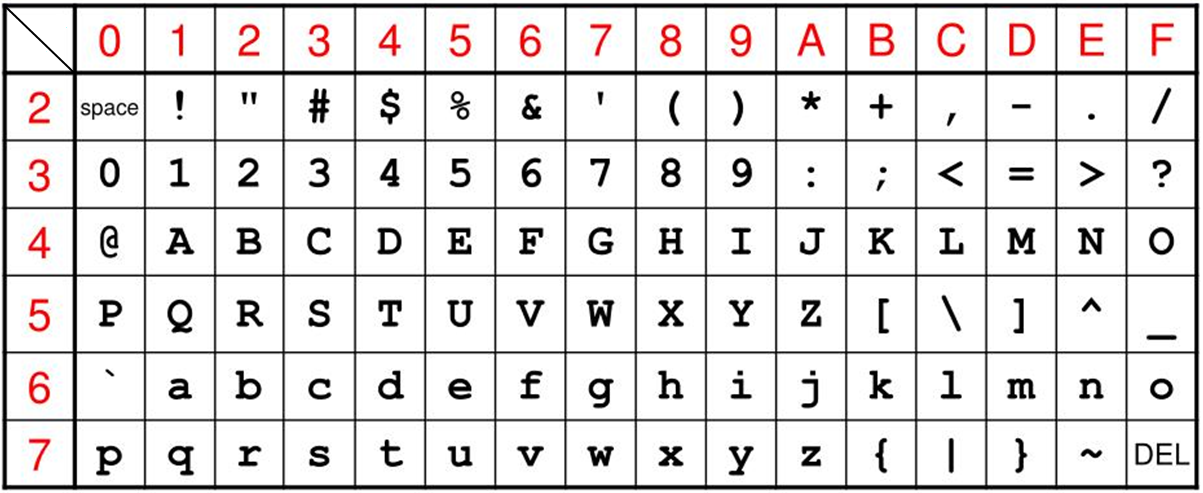
\includegraphics[width=10cm]{img/ascii}\\
            \end{center}
            \textit{\footnotesize Exemple de lecture : le caractère correspondant à l’octet codé \texttt{4A} en hexadécimal est la lettre \texttt{J}.}\\
           	\item Pour chiffrer le message d’Alice, on réalise l’opération \texttt{XOR} bit à bit avec la clé suivante :
               \begin{center}
               \texttt{k = 0b 1110 1110 1111 0000}
               \end{center}
               Donner l’écriture binaire du message obtenu.
           \end{enumerate}

       	\item 	\begin{enumerate}[\bfseries a.]
           	\item 	Donner la table de vérité de l'expression booléenne \texttt{(a XOR b) XOR b}.
           	\item 	Bob connaît la chaîne de caractères utilisée par Alice pour chiffrer le message. Quelle opération doit-il réaliser pour déchiffrer son message ?

           \end{enumerate}
       \end{enumerate}
\end{exercice}
\end{document}